% Options for packages loaded elsewhere
\PassOptionsToPackage{unicode}{hyperref}
\PassOptionsToPackage{hyphens}{url}
%
\documentclass[
]{article}
\usepackage{amsmath,amssymb}
\usepackage{iftex}
\ifPDFTeX
  \usepackage[T1]{fontenc}
  \usepackage[utf8]{inputenc}
  \usepackage{textcomp} % provide euro and other symbols
\else % if luatex or xetex
  \usepackage{unicode-math} % this also loads fontspec
  \defaultfontfeatures{Scale=MatchLowercase}
  \defaultfontfeatures[\rmfamily]{Ligatures=TeX,Scale=1}
\fi
\usepackage{lmodern}
\ifPDFTeX\else
  % xetex/luatex font selection
\fi
% Use upquote if available, for straight quotes in verbatim environments
\IfFileExists{upquote.sty}{\usepackage{upquote}}{}
\IfFileExists{microtype.sty}{% use microtype if available
  \usepackage[]{microtype}
  \UseMicrotypeSet[protrusion]{basicmath} % disable protrusion for tt fonts
}{}
\makeatletter
\@ifundefined{KOMAClassName}{% if non-KOMA class
  \IfFileExists{parskip.sty}{%
    \usepackage{parskip}
  }{% else
    \setlength{\parindent}{0pt}
    \setlength{\parskip}{6pt plus 2pt minus 1pt}}
}{% if KOMA class
  \KOMAoptions{parskip=half}}
\makeatother
\usepackage{xcolor}
\usepackage[margin=1in]{geometry}
\usepackage{graphicx}
\makeatletter
\def\maxwidth{\ifdim\Gin@nat@width>\linewidth\linewidth\else\Gin@nat@width\fi}
\def\maxheight{\ifdim\Gin@nat@height>\textheight\textheight\else\Gin@nat@height\fi}
\makeatother
% Scale images if necessary, so that they will not overflow the page
% margins by default, and it is still possible to overwrite the defaults
% using explicit options in \includegraphics[width, height, ...]{}
\setkeys{Gin}{width=\maxwidth,height=\maxheight,keepaspectratio}
% Set default figure placement to htbp
\makeatletter
\def\fps@figure{htbp}
\makeatother
\usepackage{soul}
\setlength{\emergencystretch}{3em} % prevent overfull lines
\providecommand{\tightlist}{%
  \setlength{\itemsep}{0pt}\setlength{\parskip}{0pt}}
\setcounter{secnumdepth}{-\maxdimen} % remove section numbering
\ifLuaTeX
  \usepackage{selnolig}  % disable illegal ligatures
\fi
\IfFileExists{bookmark.sty}{\usepackage{bookmark}}{\usepackage{hyperref}}
\IfFileExists{xurl.sty}{\usepackage{xurl}}{} % add URL line breaks if available
\urlstyle{same}
\hypersetup{
  pdftitle={High Poverty Rates Correspond with Mental Health Rates in New York},
  pdfauthor={Esenia Hernandez},
  hidelinks,
  pdfcreator={LaTeX via pandoc}}

\title{High Poverty Rates Correspond with Mental Health Rates in New
York}
\author{Esenia Hernandez}
\date{2023-08-07}

\begin{document}
\maketitle

\hypertarget{high-poverty-rates-correspond-with-mental-health-rates}{%
\subsection{High Poverty Rates Correspond with Mental Health
Rates}\label{high-poverty-rates-correspond-with-mental-health-rates}}

\ul{Abstract:}

Mental health impacts people all throughout the world. During the
Covid-19 pandemic, mental health rates rose significantly in New York,
especially in low-income communities. To observe how poverty affects
mental health, I used the 2020 New York Common Health Survey. This
survey has over 8,000 responses and I focused specifically on the mental
health and poverty group variables. Throughout my research, I discovered
that there is a significant difference in mental health rates among the
poverty groups, but some were also similar to each other. These findings
proved my initial hypothesis and highlighted the gaps in mental health
among poverty groups. Lastly, poverty groups two and three had the
highest rates of mental health among all groups. These results can be
used to further explore the impacts poverty has on mental health and
treatment in these groups to take action for improvement.

\ul{Background:}

In 2020, the Covid-19 pandemic had a big impact on health all over the
world. Specifically on mental health in low-income communities.
According to the New York Health Foundation, ``low-income New Yorkers
experienced the highest rates of poor mental health.'' Raising the
question, to what extent do poverty rates affect mental health and
treatment among New York residents in 2020?

\textbf{Hypothesis:} Poverty has a significant impact on mental health
among New York residents.

Overall, poverty can affect the ability to be diagnosed and receive
treatment for mental health illnesses. Through the first-hand experience
of living in a low-income community, mental health issues are often
overlooked and dismissed due to the unavailability to receive the
treatment and care needed. In order to explore the effects of poverty,
my research will be focused on studying the New York Common Health
Survey from 2020. The Common Health Survey is a computer-assisted
telephone interviewing system that is used to collect survey data from
residents 18 years old and above. This data is useful in observing a
variety of poverty groups and demographics regarding health.

\ul{Results:}

\textbf{Variable Definition Table}

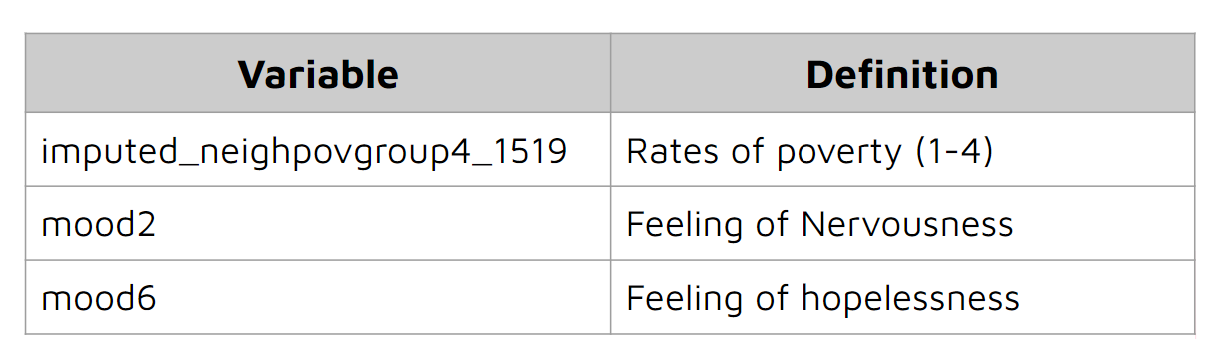
\includegraphics{images/Screenshot 2023-08-08 142431.png}

\textbf{I. Poverty Rate and Mental Health Correlation Plot}

\begin{verbatim}
## [1] "C:/Users/lunar/OneDrive/Documents/DSRP 2023/DSRP-2023-Greenleaf"
\end{verbatim}

\begin{verbatim}
## 
## Attaching package: 'dplyr'
\end{verbatim}

\begin{verbatim}
## The following objects are masked from 'package:stats':
## 
##     filter, lag
\end{verbatim}

\begin{verbatim}
## The following objects are masked from 'package:base':
## 
##     intersect, setdiff, setequal, union
\end{verbatim}

\begin{verbatim}
## -- Attaching packages -------------------------------------- tidymodels 1.1.0 --
\end{verbatim}

\begin{verbatim}
## v broom        1.0.5     v rsample      1.1.1
## v dials        1.2.0     v tibble       3.2.1
## v ggplot2      3.4.2     v tidyr        1.3.0
## v infer        1.0.4     v tune         1.1.1
## v modeldata    1.1.0     v workflows    1.1.3
## v parsnip      1.1.0     v workflowsets 1.0.1
## v purrr        1.0.1     v yardstick    1.2.0
## v recipes      1.0.6
\end{verbatim}

\begin{verbatim}
## -- Conflicts ----------------------------------------- tidymodels_conflicts() --
## x purrr::discard() masks scales::discard()
## x dplyr::filter()  masks stats::filter()
## x dplyr::lag()     masks stats::lag()
## x recipes::step()  masks stats::step()
## * Use suppressPackageStartupMessages() to eliminate package startup messages
\end{verbatim}

\begin{verbatim}
## 
## Attaching package: 'reshape2'
\end{verbatim}

\begin{verbatim}
## The following object is masked from 'package:tidyr':
## 
##     smiths
\end{verbatim}

\begin{verbatim}
## Registered S3 method overwritten by 'quantmod':
##   method            from
##   as.zoo.data.frame zoo
\end{verbatim}

\begin{verbatim}
## Warning: na_mean: No imputation performed for column 51 of the input dataset.
##                 Reason: Input x is not numeric.
\end{verbatim}

\begin{verbatim}
##   [1] X                           cid                        
##   [3] strata                      survey                     
##   [5] wt21_dual                   wt21_dual_q1               
##   [7] strata_q1                   qxvers                     
##   [9] mood1                       mood2                      
##  [11] mood3                       mood4                      
##  [13] mood5                       mood6                      
##  [15] mood9                       mood8                      
##  [17] mood11                      nutrition1                 
##  [19] newrace                     newrace6                   
##  [21] agegroup                    agegroup5                  
##  [23] agegroup6                   age21up                    
##  [25] age25up                     age40new                   
##  [27] age45up                     age50up                    
##  [29] age18_64                    birthsex                   
##  [31] imputed_neighpovgroup4_1519 imputed_povertygroup       
##  [33] imputed_povgroup3           imputed_pov200             
##  [35] generalhealth               insuredgateway20           
##  [37] insured                     insure5                    
##  [39] pcp20                       medplace                   
##  [41] didntgetcare20              regularrx                  
##  [43] skiprxcost                  toldhighbp20               
##  [45] toldprescription20          takingmeds20               
##  [47] checkedbp20_q1              diabetes20                 
##  [49] ageatdiabetes               diabcntrlmeds              
##  [51] toohighblsugar              everasthma                 
##  [53] currentasthma20             stillasthmaall             
##  [55] firsttoldasthma             k6                         
##  [57] nspd                        mhtreat20_all              
##  [59] delaypayrent                workingac_q1               
##  [61] rodentsstreet               helpneighbors20_q1         
##  [63] discussissues               helpcommproj               
##  [65] didntcleandog               trustkeys                  
##  [67] proudneigh                  smoker                     
##  [69] everyday                    numberperdaya              
##  [71] cpd20a                      heavysmoker20a             
##  [73] everydaycpda                smokecat                   
##  [75] mentholcigs20               sourcelastcig              
##  [77] cost20cigarettes            cigpurchase20              
##  [79] cigarillo20_q1              smokeecig12m20_q1          
##  [81] smokeecig30days20_q1        likedecigsflavs_q1         
##  [83] smokehookah12m_q1           smellcigsmoke20_q1         
##  [85] newrace6_b                  usborn                     
##  [87] maritalstatus20             sexualid20                 
##  [89] education                   employment20               
##  [91] emp3                        bmi                        
##  [93] weightall                   weight20in4                
##  [95] weight20in5                 fluvaccineshot             
##  [97] whereflu20                  fruitveg20                 
##  [99] avgsodaperday20             twoplussoda                
## [101] nsugardrinkperday20         avgsugarperday20           
## [103] nsodasugarperday20          avgsodasugarperday20       
## [105] ssb                         exercise20                 
## [107] cyclingfreq                 cycling20                  
## [109] swim                        difficultdailyact          
## [111] assistdevice                evercolon20                
## [113] colonoscopy10yr20           evercolon20_45             
## [115] colonoscopy10yr_45          hiv12months20              
## [117] everhivtest20               condom20                   
## [119] analsex                     analstdtest                
## [121] analsexcondomuse20          sexbehav_active20          
## [123] wsw                         wswexclusive               
## [125] sexuallyactive20            sexpartner                 
## [127] everheardofprep             everusedprep20             
## [129] msm                         msmexclusive               
## [131] bthcontrollastsex20_q1      condomusetrend             
## [133] drinker                     daysalc30                  
## [135] averagedrink20              heavydrink20               
## [137] bingenew                    ipvphy                     
## [139] insultipv                   wt_compare                 
## [141] insure20r                   hhsize                     
## [143] child                      
## <0 rows> (or 0-length row.names)
\end{verbatim}

\includegraphics{Written-Report_files/figure-latex/graph1-1.pdf}

This plot shows the correlation between poverty and mental health
variables. Based on the plot, \texttt{mood2} and \texttt{mood6} have the
highest positive correlation with poverty. These variables will be used
to compare the rates of mental health among poverty groups.

\textbf{Hypothesis Testing}

Apart from the correlation plot, t-testing, a statistical test used to
compare means, was performed to compare the mental health rates among
the wealthiest and poorest groups of residents. The t-test resulted in a
p-value of \textbf{0.02012}, demonstrating a significant difference
between the groups.

Additionally, machine learning models were developed, specifically
regression models. A boosted tree and random forest model were used to
observe any changes in poverty rate and mental health. The models
demonstrated a high percentage of errors, showing room for improvement.

\textbf{II. Frequency of Nervousness among Poverty Groups}

\begin{verbatim}
## Warning in geom_col(stat = "identity"): Ignoring unknown parameters: `stat`
\end{verbatim}

\includegraphics{Written-Report_files/figure-latex/graph2-1.pdf}

This bar graph shows how frequently feelings of nervousness were present
among poverty groups. Based on the graph, poverty groups have different
amounts of frequency.

\textbf{III. Frequency of Worthlessness among Poverty Groups}

\begin{verbatim}
## Warning in geom_col(stat = "stack"): Ignoring unknown parameters: `stat`
\end{verbatim}

\includegraphics{Written-Report_files/figure-latex/graph3-1.pdf}

This bar graph shows how frequent feelings of worthlessness were present
among poverty groups. Similar to the previous figure, poverty groups
varied in frequency.

\ul{Discussion:}

Based on the results, poverty groups two and three have the highest
rates of mental health. Demonstrating that poverty has a significant
impact on mental health and proving the hypothesis. These results can
help medical workers further research in low-income areas and create a
plan of action to help residents get the treatment needed. At first, I
expected the groups with the highest level of poverty to have the
highest rates of mental health.

However, poverty group two has significantly spiked results due to a
greater amount of people interviewed in that group. Additionally, many
of the variables from the survey dataset were not available due to
transferring issues which limited further exploration of variables.

Some next steps would be to explore the probability of substance abuse
by including different variables. As well as the further development of
machine learning models to observe changes. This research would help
determine if mental health plays a big role in drinking alcohol and
smoking in New York.

\ul{Code and Data Availability:}

Coding can be found on
\href{github.com/the-codingschool/DSRP-2023-Greenleaf/tree/main/Esenia}{GitHub}.
The New York Common Health Survey 2020 data can be found
\href{https://www.nyc.gov/site/doh/data/data-sets/community-health-survey-public-use-data.page}{here}.

\ul{Acknowledgments:}

I would like to acknowledge Columbia University professor, Dr.~Greenleaf
for mentoring me throughout my research and for helping me learn more
about public health. I would also like to acknowledge The Coding School
for granting me a full scholarship to participate in the Data Science
Research Program. Lastly, I would like to acknowledge Sarah Parker,
Yijia Wang, and Mira Bell for helping me learn all about R and fixing
bugs.

\end{document}
